%!TEX root = raspi_journal.tex
\label{sec:measurements}

This section may be divided by subheadings. It should provide a concise and
precise description of the experimental results, their interpretation as well as
the experimental conclusions that can be drawn.

\subsubsection{Multicore Network Coding}
\label{subs:multicore-network-coding}

The authors implemented the algorithm described in
Section~\ref{sub:implementation-multicore} on the Raspberry Pi 2 Model B, which
features four ARM Cortex-A7 cores in a Broadcom BCM2836 \ac{SOC} with a 900 MHz
clock. Each core has a 32 KiB L1 data cache and 32 KiB L1 instruction cache. The
cores share a 512 KiB L2 cache. All the measured results, including the baseline
results, were obtained with NEON-enabled code adopted from the FIFI/KODO library
\cite{kodo2011pedersen}. The NEON extension provides an 128-bit \ac{SIMD}
instruction set to the Raspberry Pi 2. Figures~\ref{enc_dec1024},
\ref{enc_dec128} and \ref{enc_dec16} show the encoding and decoding throughput
in MiB per second for different generation sizes ($g$ = 1024, 128, and 16
respectively). The throughput is the rate of generating $g$ coded packets,
divided by the time the encoder took to perform the task. The size of each coded
packet was fixed to $1536$~bytes since that is the typical size of an Ethernet
frame. The blocked operations were performed dividing the matrices in squared
sub-blocks of 16,32,64,...,1024 operands (words in the finite field) in height
and width, and the figures only show the best results (usually block sizes of
16x16 or 32x32 operands since with bigger block sizes, the operands do not fit
in L1 cache).

The following test cases were considered:

\paragraph{Baseline encoding} The baseline results involve no recording of the
\ac{DAG} and are performed in a \emph{by-the-book} fashion. The encoder uses
only one thread. And the difference between the non-blocked and blocked encoding
schemes is that in the blocked scheme, the matrix multiplications are performed
dividing the matrices in sub-blocks in order to make the algorithm cache
efficient as described in Section~\ref{sub:implementation-multicore}.

\paragraph{Encoding blocked} The encoding results were performed using the
method described in Section~\ref{sub:implementation-multicore}. The time
recorded includes the dependencies resolving, creation of the \ac{DAG}, and the
task scheduling. In practice, it would suffice to calculate and store this
information only once per generation size.

\paragraph{Decoding blocked} The differences between encoding and decoding, is
that the decoding task also involves the matrix inversion. Similarly as with the
encoding results, the time recorded includes the dependencies resolving, the
creation of the \ac{DAG} and the task scheduling. However, to decode, these
calculations are also made for inverting the matrix of coding coefficients.

\begin{figure}[h!]
\centering
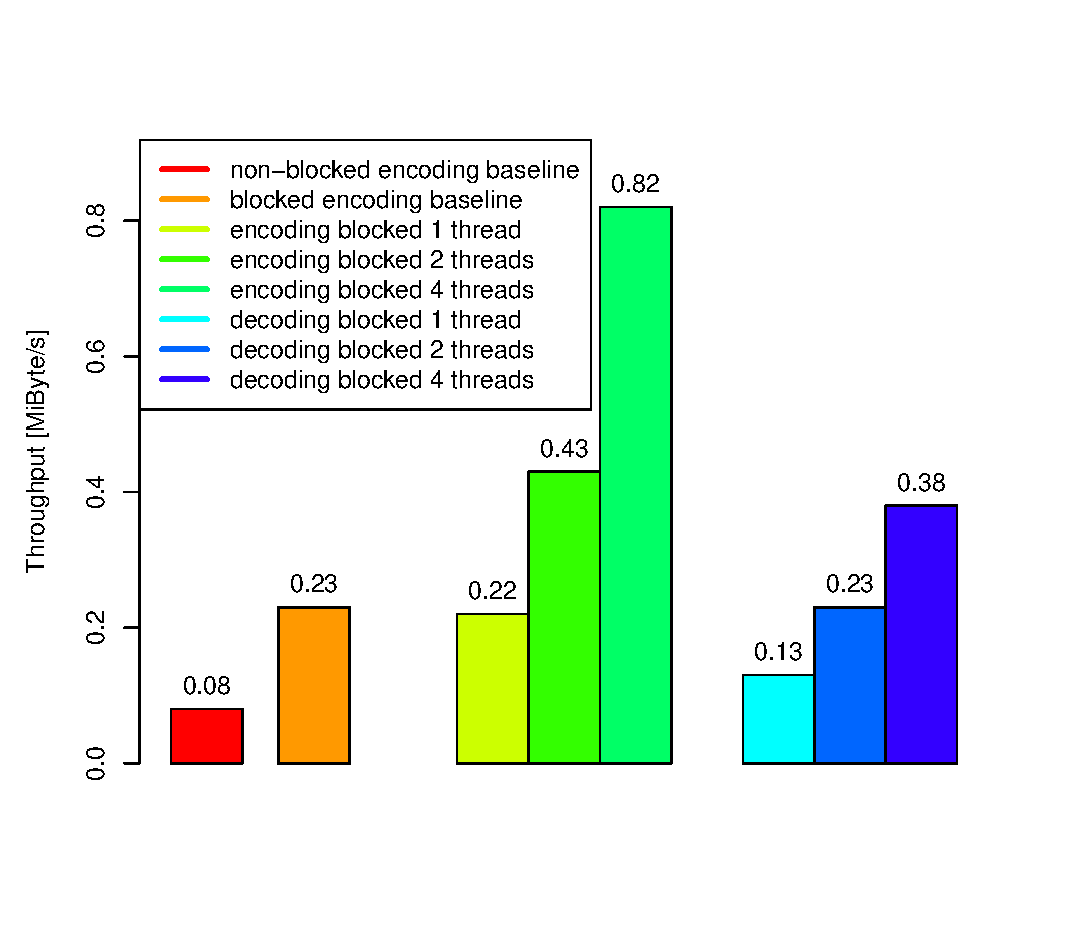
\includegraphics[width=0.5\textwidth]{images/2015-04-18_encoding_decoding_1024.eps}
\caption{Encoding and Decoding performance for g = 1024 \cite{wunderlich2015network}}
\label{enc_dec1024}
\end{figure}

For $g=$ 1024, the blocked baseline measurements outperforms the non blocked
variant. This means that making the matrix multiplication algorithm cache
efficient brings an increase in throughput by a factor of 2.83. When using the
algorithm described in Section~\ref{sub:implementation-multicore}, encoding with
four cores is on average 3.7 times faster than with one core. Similarly,
decoding with four codes is 3.05 times faster, on average, than decoding with a
single core. Figure~\ref{enc_dec1024} shows that the implemented algorithm, by
exploiting cache efficiency and only three extra cores provides a gain of 10
folds compared with traditional non-blocked algorithms. With $g$ = 1024, the
matrix inversion becomes more expensive than at smaller generations sizes.
Therefore, the decoding throughput is 46\% of the encoding throughput.

\begin{figure}[h!]
\centering
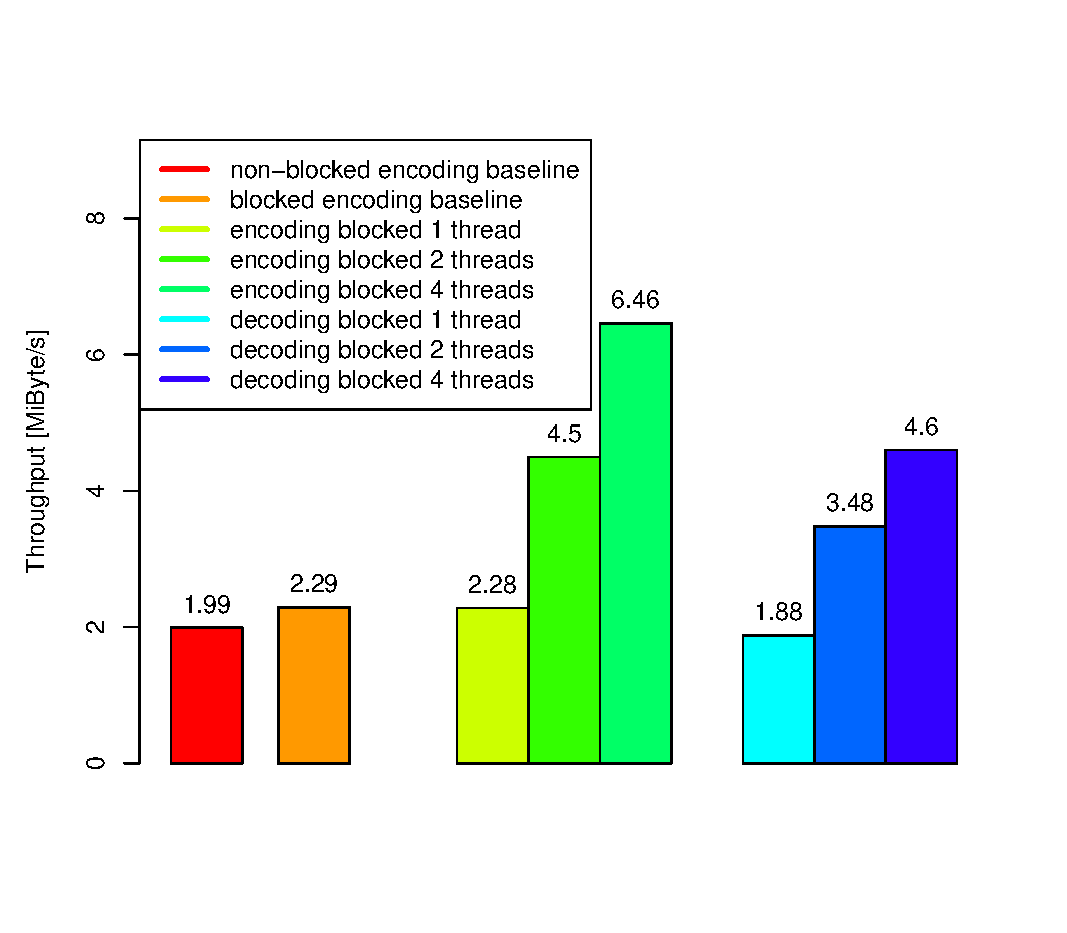
\includegraphics[width=0.5\textwidth]{images/2015-04-18_encoding_decoding_128.eps}
\caption{Encoding and Decoding performance for g = 128 \cite{wunderlich2015network}}
\label{enc_dec128}
\end{figure}

For $g$ = 128, the differences between the baselines operations show that a
blocked algorithm is 15\% faster than the non-blocked variant. Encoding with
four cores is 2.82 times faster than with a single core. Due to the smaller
matrix sizes, the gain when using blocked operations in the baselines is not
that significant when compared with $g$ = 1024. For the same reason, the matrix
inversion is less expensive. As a consequence, the decoding throughput is 71\%
of the encoding throughput.

\begin{figure}[h!]
\centering
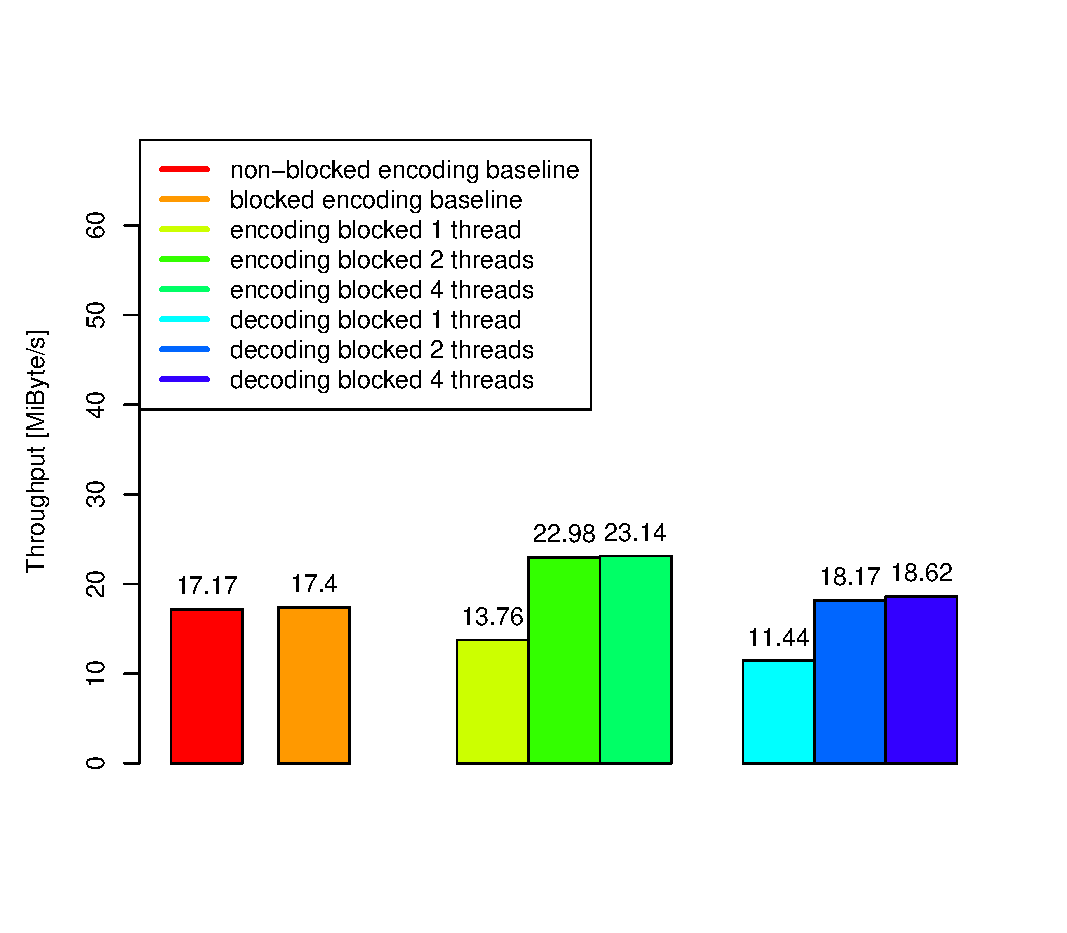
\includegraphics[width=0.5\textwidth]{images/2015-04-18_encoding_decoding_16.eps}
\caption{Encoding and Decoding performance for g = 16 \cite{wunderlich2015network}}
\label{enc_dec16}
\end{figure}

When $g$ = 16, the gains of blocked operations are negligible compared with the
non-blocked ones. The reason behind this behavior is that all the data fits in
the L1 cache. For the scheduled version, since the problem to solve is so small,
the gain when using four cores is a factor of 1.68 compared with a single core,
and 1.01 compared with two cores. Therefore, there are no practical benefits in
using four cores instead of two.

The differences in throughput, for all generation sizes, between the blocked
baseline and the single threaded scheduled measurements are due the time spent
resolving the dependencies and the scheduling overhead. These effects are
negligible for big generation sizes, while considerable for small matrices.

% \begin{figure}
% \centering
% \begin{subfigure}[b]{0.3\textwidth}
% 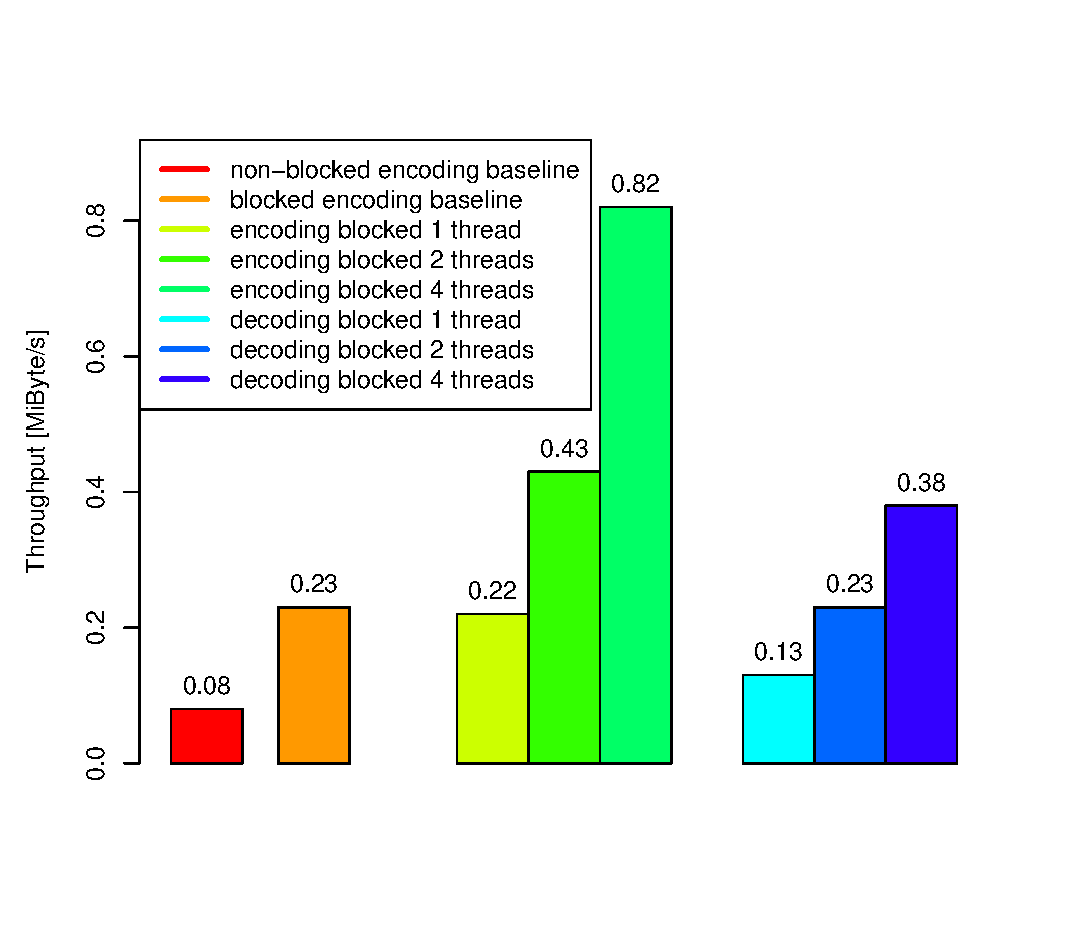
\includegraphics[width=\textwidth]{images/2015-04-18_encoding_decoding_1024.eps}
% \caption{Encoding and Decoding performance for g = 1024}
% \label{enc_dec1024}
% \end{subfigure}
%
% \begin{subfigure}[b]{0.3\textwidth}
% 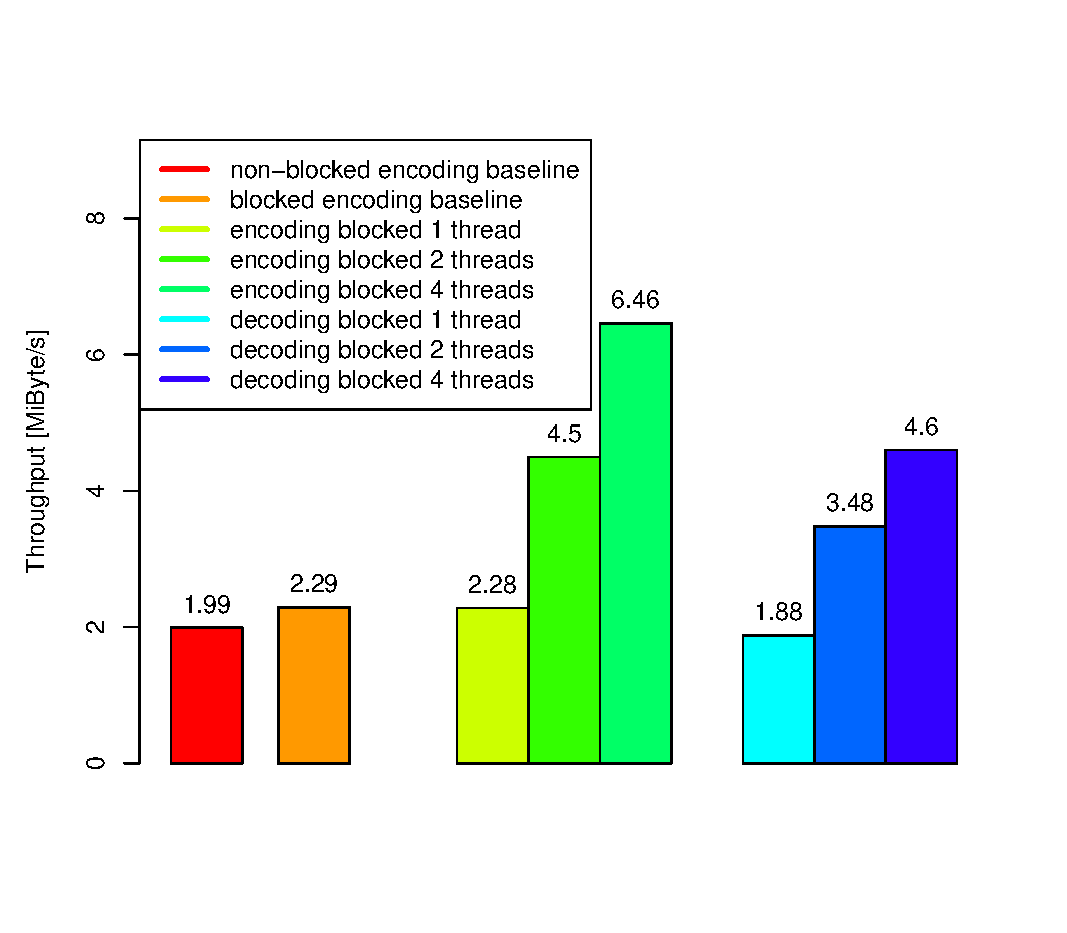
\includegraphics[width=\textwidth]{images/2015-04-18_encoding_decoding_128.eps}
% \caption{Encoding and Decoding performance for g = 128}
% \label{enc_dec128}
% \end{subfigure}
%
% \begin{subfigure}[b]{0.3\textwidth}
% 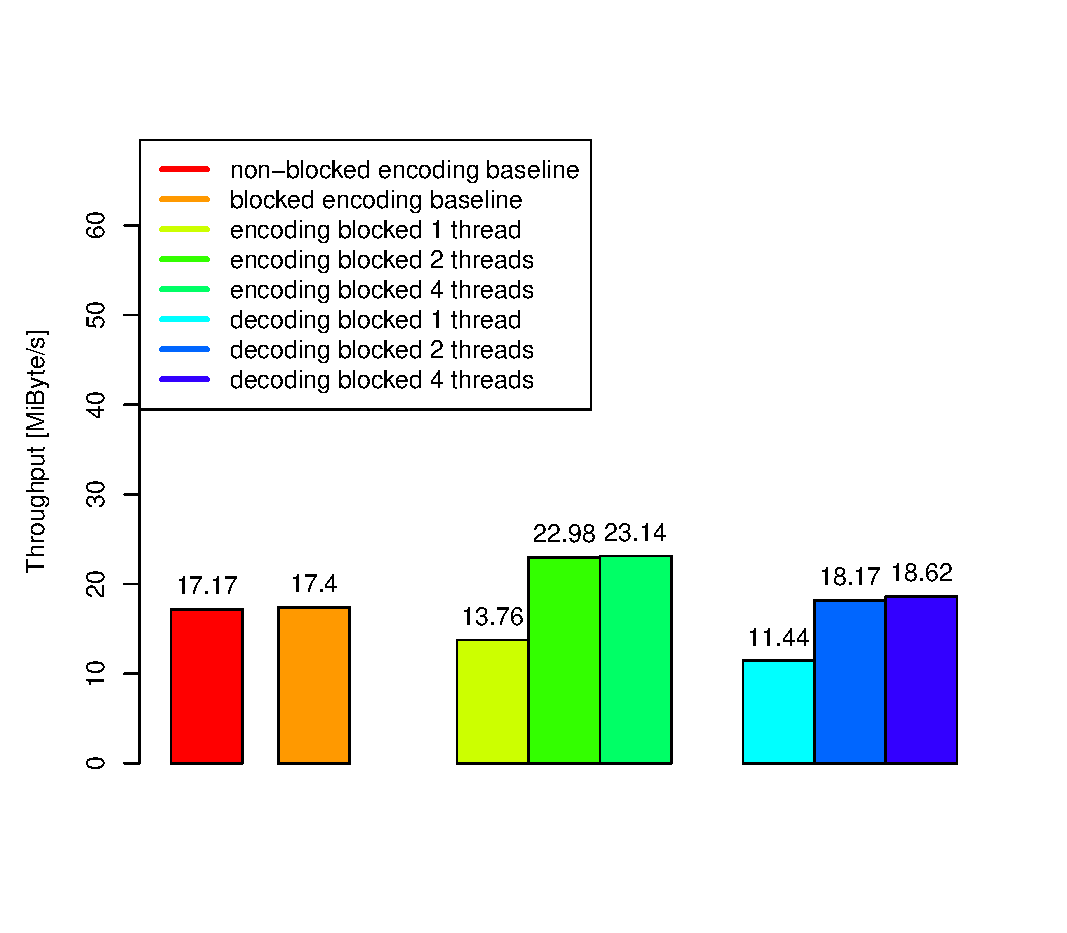
\includegraphics[width=\textwidth]{images/2015-04-18_encoding_decoding_16.eps}
% \caption{Encoding and Decoding performance for g = 16}
% \label{enc_dec16}
% \end{subfigure}
% \end{figure}



\paragraph{Comparison of the load of matrix multiplications and inversions}

To compare how much slower is the matrix multiplication with respect to the
matrix inversion for different generation sizes, we ran a set of tests. We used
a single core to perform the operations. We changed the generation sizes,
performed matrices multiplications and matrix inversions, and measured the time
spent doing so. We then calculated the ratio between these two measured times
times $ratio = \frac{T_{mult}}{T_{inv}}$. Table~\ref{runtimes} summarizes the
results. The bigger the matrix size, the smaller is the calculated ratio. This
means that when the problems are bigger, the decoding throughput decreases
compared with the encoding throughput.

\begin{table}[H]
\center
\caption{Multiplication and inversion run-times for different generation sizes with 1 thread}
\begin{tabular}{|r|r|r|r|}
\hline
g & multiplication (ms) & inversion (ms) & ratio \\
\hline
\hline

	16 & 1.703  & 0.345 & 4.9 \\
\hline
	32 & 6.573  & 0.914 & 7.2 \\
\hline
	64 & 21.341  & 3.479 & 6.1 \\
\hline
	128 & 82.326  & 17.411 & 4.7 \\
\hline
	256 & 336.398  & 106.861 & 3.1 \\
\hline
	512 & 1548.750  & 659.469 & 2.3 \\
\hline
	1024 & 6730.380  & 5166.920 & 1.3 \\
\hline
\end{tabular}
\vspace{0.2cm}
\label{runtimes}
\end{table}
